\documentclass[tikz,border=1.0mm]{standalone}
\usepackage{fontspec,amsmath,amssymb,xcolor,lmodern}
\setsansfont{Arial}
\usetikzlibrary{arrows.meta,positioning,calc,fit,backgrounds,patterns,decorations.pathreplacing,shapes.geometric}

% High-Contrast Deep Top-Journal Palette (Nature Biotech / IEEE TPAMI / OriginPro Ink)
\definecolor{Ink}{HTML}{0F172A}
\definecolor{Crimson}{HTML}{B91C1C}
\definecolor{Carmine}{HTML}{DC2626}
\definecolor{Navy}{HTML}{1D4ED8}
\definecolor{DeepNavy}{HTML}{1E3A8A}
\definecolor{Violet}{HTML}{5B21B6}
\definecolor{DeepViol}{HTML}{4C1D95}
\definecolor{Emerald}{HTML}{047857}
\definecolor{Teal}{HTML}{0F766E}
\definecolor{Amber}{HTML}{B45309}
\definecolor{Gold}{HTML}{D97706}
\definecolor{Plum}{HTML}{9D174D}
\definecolor{Slate}{HTML}{334155}
\definecolor{Muted}{HTML}{64748B}

% Crisp Structural Tints (High-contrast borders, subtle architectural fills)
\definecolor{ZoneBlue}{HTML}{EFF6FF}
\definecolor{ZoneViol}{HTML}{F5F3FF}
\definecolor{ZoneEm}{HTML}{ECFDF5}
\definecolor{ZoneRed}{HTML}{FEF2F2}
\definecolor{ZoneAmb}{HTML}{FFFBEB}
\definecolor{ZoneGray}{HTML}{F8FAFC}
\definecolor{GridLine}{HTML}{CBD5E1}

\begin{document}
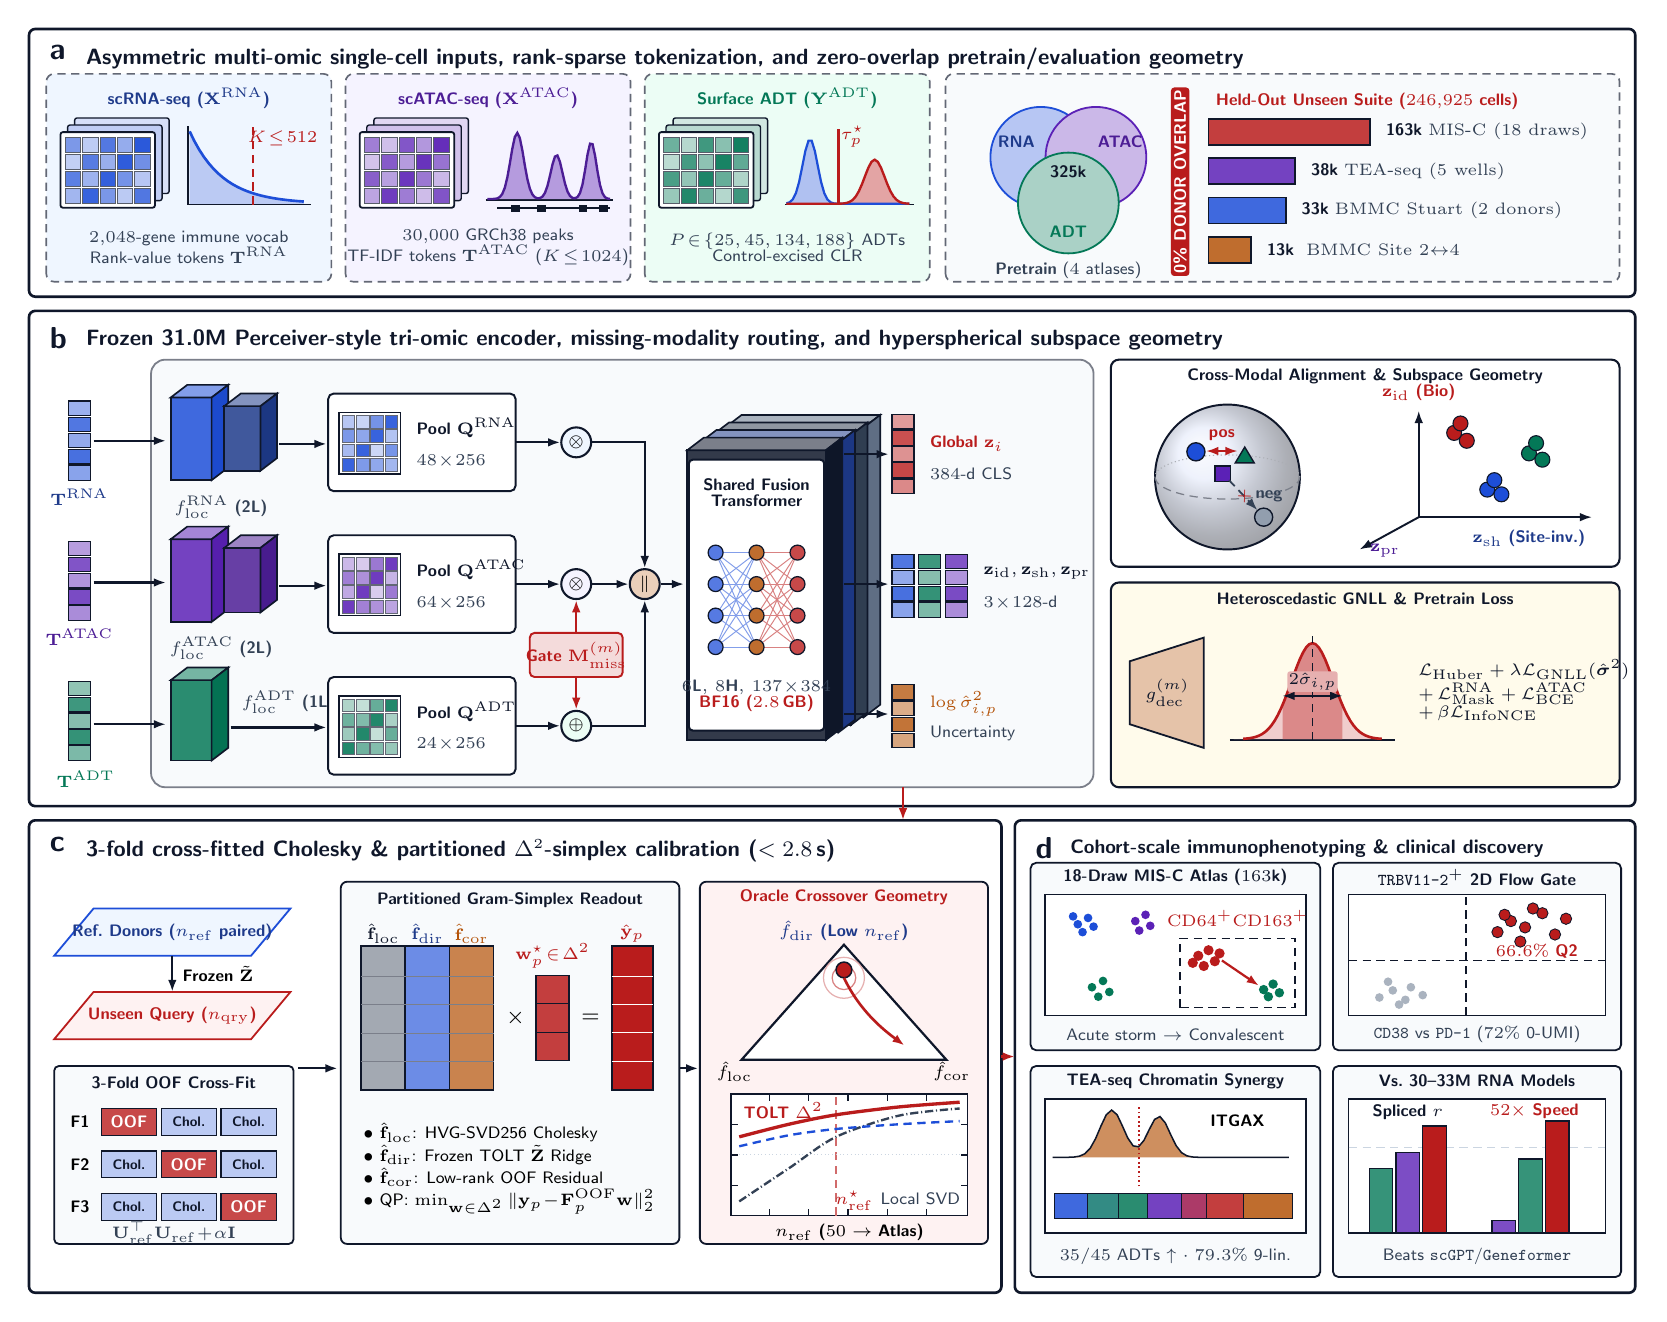
\begin{tikzpicture}[
  x=1mm, y=1mm,
  >={Latex[length=1.55mm,width=1.10mm]},
  panel/.style={draw=Ink, line width=0.95pt, rounded corners=0.8mm, fill=white},
  subzone/.style={draw=Ink!65, line width=0.60pt, densely dashed, rounded corners=1.0mm},
  flow/.style={->, draw=Ink, line width=0.80pt},
  flowred/.style={->, draw=Crimson, line width=0.85pt},
  opnode/.style={circle, draw=Ink, line width=0.75pt, inner sep=0pt, minimum size=3.8mm, font=\sffamily\bfseries\fontsize{6.4}{6.8}\selectfont},
  pletter/.style={font=\sffamily\bfseries\fontsize{11.0}{11.5}\selectfont, text=Ink, anchor=north west},
  ptitle/.style={font=\sffamily\bfseries\fontsize{8.2}{9.0}\selectfont, text=Ink, anchor=north west},
  lbl/.style={font=\sffamily\bfseries\fontsize{6.4}{7.1}\selectfont, text=Ink, align=center},
  sublbl/.style={font=\sffamily\fontsize{5.8}{6.5}\selectfont, text=Slate, align=center}
]

% --- Reusable Visual Macros ---
% 1) Overlapping 3-Deck Cell-by-Feature Heatmap Matrix (#1=x, #2=y, #3=BaseColor)
\newcommand{\MatrixDeck}[3]{
  \filldraw[fill=#3!18, draw=Ink, line width=0.50pt, rounded corners=0.3mm] (#1+1.8,#2+1.8) rectangle ++(12.0,9.6);
  \filldraw[fill=#3!28, draw=Ink, line width=0.50pt, rounded corners=0.3mm] (#1+0.9,#2+0.9) rectangle ++(12.0,9.6);
  \filldraw[fill=white, draw=Ink, line width=0.65pt, rounded corners=0.3mm] (#1,#2) rectangle ++(12.0,9.6);
  \foreach \r in {0,...,3}{
    \foreach \c in {0,...,4}{
      \pgfmathsetmacro{\sh}{int(22 + mod(\r*31 + \c*47 + 19, 76))}
      \filldraw[fill=#3!\sh!white, draw=Ink!70, line width=0.25pt]
        (#1+0.6+\c*2.2, #2+0.6+\r*2.15) rectangle ++(1.95,1.85);
    }
  }
}

% 2) 3D Isometric Encoder Slab (#1=x, #2=y, #3=w, #4=h, #5=Color)
\newcommand{\IsoSlab}[5]{
  \pgfmathsetmacro{\dx}{2.1}
  \pgfmathsetmacro{\dy}{1.6}
  \filldraw[fill=#5!85!white, draw=Ink, line width=0.60pt]
    (#1,#2) rectangle ++(#3,#4);
  \filldraw[fill=#5!55!white, draw=Ink, line width=0.60pt]
    (#1,#2+#4) -- ++(\dx,\dy) -- ++(#3,0) -- (#1+#3,#2+#4) -- cycle;
  \filldraw[fill=#5!95!black, draw=Ink, line width=0.60pt]
    (#1+#3,#2) -- ++(\dx,\dy) -- ++(0,#4) -- (#1+#3,#2+#4) -- cycle;
}

% 3) Token Vector Strip (#1=x, #2=y, #3=N, #4=Color)
\newcommand{\TokStrip}[4]{
  \foreach \k in {0,...,#3}{
    \pgfmathsetmacro{\sh}{int(35 + mod(\k*29+17, 62))}
    \filldraw[fill=#4!\sh!white, draw=Ink, line width=0.42pt]
      (#1, #2+\k*2.05) rectangle ++(2.8,1.85);
  }
}

% 4) Attention Q x K^T Heatmap Grid (#1=x, #2=y, #3=Color)
\newcommand{\AttnGrid}[3]{
  \filldraw[fill=white, draw=Ink, line width=0.55pt] (#1,#2) rectangle ++(7.8,7.8);
  \foreach \r in {0,...,3}{
    \foreach \c in {0,...,3}{
      \pgfmathsetmacro{\sh}{int((\r==\c ? 88 : 20 + mod(\r*19+\c*37, 45)))}
      \filldraw[fill=#3!\sh!white, draw=Ink!65, line width=0.22pt]
        (#1+0.35+\c*1.82, #2+0.35+\r*1.82) rectangle ++(1.62,1.62);
    }
  }
}

% =========================================================================
% PANEL A (TOP): MULTI-OMIC SINGLE-CELL TENSORS & DISJOINT CORPUS GEOMETRY
% =========================================================================
\draw[panel] (1.0,127.5) rectangle (205.0,161.5);
\node[pletter] at (2.4,160.6) {a};
\node[ptitle] at (7.0,160.3) {Asymmetric multi-omic single-cell inputs, rank-sparse tokenization, and zero-overlap pretrain/evaluation geometry};

% --- A1: Three Visual Modality Decks + Signal Waveforms (Left, x=3..115) ---
% 1. scRNA-seq Deck
\filldraw[subzone, fill=ZoneBlue] (3.2,129.4) rectangle (39.4,155.8);
\node[lbl, text=DeepNavy] at (21.3,152.7) {scRNA-seq ($\mathbf{X}^{\mathrm{RNA}}$)};
\MatrixDeck{5.0}{138.8}{Navy}
% Rank decay curve icon
\draw[draw=Ink, line width=0.55pt] (21.2,139.2) -- (21.2,149.2);
\draw[draw=Ink, line width=0.55pt] (21.2,139.2) -- (36.8,139.2);
\fill[Navy!30] (21.4,139.3) -- plot[domain=0:14.5, samples=25] (21.4+\x, {139.3 + 9.2*exp(-0.24*\x)}) -- (35.9,139.3) -- cycle;
\draw[Navy, line width=0.95pt] plot[domain=0:14.5, samples=25] (21.4+\x, {139.3 + 9.2*exp(-0.24*\x)});
\draw[Crimson, densely dashed, line width=0.65pt] (29.5,139.2) -- (29.5,149.2);
\node[font=\sffamily\bfseries\fontsize{5.6}{6.1}\selectfont, text=Crimson] at (33.2,147.6) {$K\!\le\!512$};
\node[sublbl] at (21.3,133.8) {$2{,}048$-gene immune vocab\\[-0.2mm]Rank-value tokens $\mathbf{T}^{\mathrm{RNA}}$};

% 2. scATAC-seq Deck + Chromatin Peak Track
\filldraw[subzone, fill=ZoneViol] (41.2,129.4) rectangle (77.4,155.8);
\node[lbl, text=DeepViol] at (59.3,152.7) {scATAC-seq ($\mathbf{X}^{\mathrm{ATAC}}$)};
\MatrixDeck{43.0}{138.8}{Violet}
% Smooth cis-chromatin accessibility peaks
\draw[draw=Ink, line width=0.55pt] (59.0,139.8) -- (75.2,139.8);
\fill[Violet!45] (59.2,139.9)
  -- plot[domain=0:15.6, samples=50] (59.2+\x, {139.9 + 8.4*exp(-(\x-3.8)^2/1.4) + 5.6*exp(-(\x-8.8)^2/1.1) + 7.2*exp(-(\x-13.2)^2/0.9)})
  -- (74.8,139.9) -- cycle;
\draw[DeepViol, line width=0.85pt]
  plot[domain=0:15.6, samples=50] (59.2+\x, {139.9 + 8.4*exp(-(\x-3.8)^2/1.4) + 5.6*exp(-(\x-8.8)^2/1.1) + 7.2*exp(-(\x-13.2)^2/0.9)});
\foreach \ex in {62.2, 65.5, 70.8, 73.4}{\fill[Ink] (\ex,138.3) rectangle ++(1.1,0.9);}
\draw[Ink, line width=0.45pt] (60.5,138.75) -- (74.8,138.75);
\node[sublbl] at (59.3,133.8) {$30{,}000$ GRCh38 peaks\\[-0.2mm]TF-IDF tokens $\mathbf{T}^{\mathrm{ATAC}}$ ($K\!\le\!1024$)};

% 3. Surface Proteome Deck + Bimodal CLR Curve
\filldraw[subzone, fill=ZoneEm] (79.2,129.4) rectangle (115.4,155.8);
\node[lbl, text=Emerald] at (97.3,152.7) {Surface ADT ($\mathbf{Y}^{\mathrm{ADT}}$)};
\MatrixDeck{81.0}{138.8}{Emerald}
% Bimodal CLR density icon
\draw[draw=Ink, line width=0.55pt] (97.0,139.2) -- (113.4,139.2);
\fill[Navy!35] (97.2,139.3) -- plot[domain=0:15.6, samples=40] (97.2+\x, {139.3 + 8.2*exp(-(\x-3.0)^2/1.8)}) -- (112.8,139.3) -- cycle;
\fill[Crimson!40] (97.2,139.3) -- plot[domain=0:15.6, samples=40] (97.2+\x, {139.3 + 5.6*exp(-(\x-11.2)^2/3.2)}) -- (112.8,139.3) -- cycle;
\draw[Navy, line width=0.80pt] plot[domain=0:15.6, samples=40] (97.2+\x, {139.3 + 8.2*exp(-(\x-3.0)^2/1.8)});
\draw[Crimson, line width=0.85pt] plot[domain=0:15.6, samples=40] (97.2+\x, {139.3 + 5.6*exp(-(\x-11.2)^2/3.2)});
\draw[Crimson, line width=0.85pt] (103.8,139.2) -- (103.8,148.8);
\node[font=\sffamily\bfseries\fontsize{5.7}{6.2}\selectfont, text=Crimson] at (105.6,147.8) {$\tau_p^{\star}$};
\node[sublbl] at (97.3,133.8) {$P\!\in\!\{25,45,134,188\}$ ADTs\\[-0.2mm]Control-excised CLR};

% --- A2: Tri-Omic Venn Diagram + Disjoint Benchmark Bars (Right, x=117..203) ---
\filldraw[subzone, fill=ZoneGray] (117.4,129.4) rectangle (203.0,155.8);
% 3-Circle Euler / Venn Diagram (Reference Image 1a style!)
\begin{scope}
  \fill[Navy!32, draw=Navy, line width=0.65pt] (129.5,145.2) circle (6.4);
  \fill[Violet!32, draw=Violet, line width=0.65pt] (136.5,145.2) circle (6.4);
  \fill[Emerald!34, draw=Emerald, line width=0.65pt] (133.0,139.4) circle (6.4);
  \node[font=\sffamily\bfseries\fontsize{5.9}{6.5}\selectfont, text=DeepNavy] at (126.4,147.2) {RNA};
  \node[font=\sffamily\bfseries\fontsize{5.9}{6.5}\selectfont, text=DeepViol] at (139.6,147.2) {ATAC};
  \node[font=\sffamily\bfseries\fontsize{5.9}{6.5}\selectfont, text=Emerald] at (133.0,135.8) {ADT};
  \node[font=\sffamily\bfseries\fontsize{6.0}{6.5}\selectfont, text=Ink] at (133.0,143.4) {325k};
\end{scope}
\node[sublbl] at (133.0,130.9) {\textbf{Pretrain} ($4$ atlases)};

% Disjoint Firewall
\draw[Crimson, line width=1.0pt, densely dashed] (147.2,130.6) -- (147.2,153.6);
\node[fill=Crimson, text=white, rounded corners=0.4mm, inner sep=0.9pt, font=\sffamily\bfseries\fontsize{5.6}{6.1}\selectfont, rotate=90] at (147.2,142.1) {0\% DONOR OVERLAP};

% Proportional Horizontal Stacked/Bar Visual for 4 Held-Out Cohorts (246,925 unseen cells)
\node[lbl, text=Crimson, anchor=west] at (150.5,152.3) {Held-Out Unseen Suite ($246{,}925$ cells)};
\foreach \y/\w/\col/\nm/\ct in {
  146.8/20.5/Crimson/MIS-C (18 draws)/163k,
  141.8/11.0/Violet/TEA-seq (5 wells)/38k,
  136.8/9.8/Navy/BMMC Stuart (2 donors)/33k,
  131.8/5.4/Amber/BMMC Site 2$\leftrightarrow$4/13k
}{
  \filldraw[fill=\col!85!white, draw=Ink, line width=0.60pt] (150.8,\y) rectangle ++(\w,3.3);
  \node[font=\sffamily\bfseries\fontsize{5.6}{6.0}\selectfont, text=Ink, anchor=west] at (151.6+\w,\y+1.65) {\ct\ {\normalfont\color{Slate}\nm}};
}

% =========================================================================
% PANEL B (CENTER HERO): 31.0M PERCEIVER TRI-OMIC ARCHITECTURE & HYPERSPHERE
% =========================================================================
\draw[panel] (1.0,62.8) rectangle (205.0,125.7);
\node[pletter] at (2.4,124.8) {b};
\node[ptitle] at (7.0,124.5) {Frozen 31.0M Perceiver-style tri-omic encoder, missing-modality routing, and hyperspherical subspace geometry};

% Soft Tinted Architectural Capsule (IEEE TPAMI Mixture-of-Views visual hierarchy!)
\filldraw[fill=ZoneGray, draw=Ink!55, line width=0.65pt, rounded corners=1.8mm] (16.5,65.2) rectangle (136.2,119.5);

% --- B1: Input Token Strips (x=4..14) ---
\TokStrip{6.0}{104.2}{4}{Navy}
\node[lbl, text=DeepNavy] at (7.4,102.0) {$\mathbf{T}^{\mathrm{RNA}}$};
\TokStrip{6.0}{86.4}{4}{Violet}
\node[lbl, text=DeepViol] at (7.4,84.2) {$\mathbf{T}^{\mathrm{ATAC}}$};
\TokStrip{6.0}{68.6}{4}{Emerald}
\node[lbl, text=Emerald] at (8.2,66.2) {$\mathbf{T}^{\mathrm{ADT}}$};

\draw[flow] (9.2,109.2) -- (18.4,109.2);
\draw[flow] (9.2,91.2) -- (18.4,91.2);
\draw[flow] (9.2,73.2) -- (18.4,73.2);

% --- B2: 3D Isometric Multi-Layer Pre-LN Encoders (Image 5 3D CNN/Transformer style!) ---
\IsoSlab{19.0}{104.2}{5.2}{10.5}{Navy}
\IsoSlab{25.8}{105.4}{4.6}{8.2}{DeepNavy}
\node[sublbl, font=\sffamily\bfseries\fontsize{5.9}{6.5}\selectfont] at (25.4,100.8) {$f_{\mathrm{loc}}^{\mathrm{RNA}}$ (2L)};

\IsoSlab{19.0}{86.2}{5.2}{10.5}{Violet}
\IsoSlab{25.8}{87.4}{4.6}{8.2}{DeepViol}
\node[sublbl, font=\sffamily\bfseries\fontsize{5.9}{6.5}\selectfont] at (25.4,82.8) {$f_{\mathrm{loc}}^{\mathrm{ATAC}}$ (2L)};

\IsoSlab{19.0}{68.6}{5.2}{10.2}{Emerald}
\node[sublbl, font=\sffamily\bfseries\fontsize{5.9}{6.5}\selectfont, anchor=west] at (26.8,76.0) {$f_{\mathrm{loc}}^{\mathrm{ADT}}$ (1L)};

\draw[flow] (32.8,108.8) -- (38.8,108.8);
\draw[flow] (32.8,90.8) -- (38.8,90.8);
\draw[flow] (26.6,72.8) -- (38.8,72.8);

% --- B3: Perceiver Cross-Attention Query Poolers with Visual Q x K^T Grids ---
\filldraw[fill=white, draw=Ink, line width=0.70pt, rounded corners=0.7mm] (39.0,102.8) rectangle (62.8,115.2);
\AttnGrid{40.4}{105.0}{Navy}
\node[lbl, anchor=west] at (49.0,110.8) {Pool $\mathbf{Q}^{\mathrm{RNA}}$};
\node[sublbl, anchor=west] at (49.0,106.6) {$48\!\times\!256$};

\filldraw[fill=white, draw=Ink, line width=0.70pt, rounded corners=0.7mm] (39.0,84.8) rectangle (62.8,97.2);
\AttnGrid{40.4}{87.0}{Violet}
\node[lbl, anchor=west] at (49.0,92.8) {Pool $\mathbf{Q}^{\mathrm{ATAC}}$};
\node[sublbl, anchor=west] at (49.0,88.6) {$64\!\times\!256$};

\filldraw[fill=white, draw=Ink, line width=0.70pt, rounded corners=0.7mm] (39.0,66.8) rectangle (62.8,79.2);
\AttnGrid{40.4}{69.0}{Emerald}
\node[lbl, anchor=west] at (49.0,74.8) {Pool $\mathbf{Q}^{\mathrm{ADT}}$};
\node[sublbl, anchor=west] at (49.0,70.6) {$24\!\times\!256$};

% --- B4: Missing-Modality Gated Router ---
\node[opnode, fill=ZoneBlue] (g1) at (70.5,109.0) {$\otimes$};
\node[opnode, fill=ZoneViol] (g2) at (70.5,91.0) {$\otimes$};
\node[opnode, fill=ZoneEm]   (g3) at (70.5,73.0) {$\oplus$};
\filldraw[fill=Crimson!16, draw=Crimson, line width=0.70pt, rounded corners=0.6mm] (64.6,79.2) rectangle (76.4,84.8);
\node[font=\sffamily\bfseries\fontsize{6.1}{6.6}\selectfont, text=Crimson, align=center] at (70.5,82.0) {Gate $\mathbf{M}_{\mathrm{miss}}^{(m)}$};
\draw[flowred] (70.5,84.8) -- (g2.south);
\draw[flowred] (70.5,79.2) -- (g3.north);
\draw[flow] (62.8,109.0) -- (g1.west);
\draw[flow] (62.8,91.0) -- (g2.west);
\draw[flow] (62.8,73.0) -- (g3.west);

\node[opnode, fill=Amber!28] (cat) at (79.2,91.0) {$\Vert$};
\draw[flow] (g1.east) -| (cat.north);
\draw[flow] (g2.east) -- (cat.west);
\draw[flow] (g3.east) -| (cat.south);

% --- B5: 6-Layer 3D Isometric Shared Fusion Perceiver-Transformer Stack ---
\draw[flow] (cat.east) -- (84.2,91.0);
\foreach \shf/\colsl in {4.8/Muted, 3.2/Slate, 1.6/DeepNavy, 0.0/Ink}{
  \IsoSlab{84.6+\shf}{71.2+\shf*0.6}{17.6}{36.8}{\colsl}
}
% Overlay clean white core card on front slab showing Bipartite Self-Attention Network
\filldraw[fill=white, draw=Ink, line width=0.75pt, rounded corners=0.5mm] (84.8,72.4) rectangle (102.0,106.8);
\node[lbl, font=\sffamily\bfseries\fontsize{5.9}{6.5}\selectfont] at (93.4,102.6) {Shared Fusion\\[-0.2mm]Transformer};
% Bipartite multi-head attention web
\foreach \ya in {83,87,91,95}{
  \foreach \yb in {83,87,91,95}{
    \draw[Navy!55, line width=0.35pt] (88.2,\ya) -- (93.4,\yb);
    \draw[Crimson!55, line width=0.35pt] (93.4,\ya) -- (98.6,\yb);
  }
}
\foreach \ya in {83,87,91,95}{
  \filldraw[fill=Navy!75, draw=Ink, line width=0.45pt] (88.2,\ya) circle (0.95);
  \filldraw[fill=Amber!85, draw=Ink, line width=0.45pt] (93.4,\ya) circle (0.95);
  \filldraw[fill=Crimson!80, draw=Ink, line width=0.45pt] (98.6,\ya) circle (0.95);
}
\node[sublbl, font=\sffamily\bfseries\fontsize{5.6}{6.1}\selectfont] at (93.4,76.8) {$6\text{L},\,8\text{H},\,137\!\times\!384$\\[-0.2mm]\color{Crimson}BF16 ($2.8$\,GB)};

% --- B6: Three Factorized Output Heads (x=108..135) ---
\draw[flow] (104.5,107.5) -- (110.2,107.5);
\draw[flow] (104.5,91.0) -- (110.2,91.0);
\draw[flow] (104.5,74.5) -- (110.2,74.5);

\TokStrip{110.6}{102.5}{4}{Crimson}
\node[lbl, anchor=west, text=Crimson] at (114.2,108.8) {Global $\mathbf{z}_i$};
\node[sublbl, anchor=west] at (114.2,105.0) {$384$-d CLS};

\TokStrip{110.6}{86.8}{3}{Navy}
\TokStrip{114.0}{86.8}{3}{Emerald}
\TokStrip{117.4}{86.8}{3}{Violet}
\node[lbl, anchor=west] at (121.0,92.4) {$\mathbf{z}_{\mathrm{id}},\mathbf{z}_{\mathrm{sh}},\mathbf{z}_{\mathrm{pr}}$};
\node[sublbl, anchor=west] at (121.0,88.6) {$3\!\times\!128$-d};

\TokStrip{110.6}{70.2}{3}{Amber}
\node[lbl, anchor=west, text=Amber] at (114.2,75.8) {$\log\hat{\sigma}_{i,p}^2$};
\node[sublbl, anchor=west] at (114.2,72.0) {Uncertainty};

% --- B7: Visual Hyperspherical Contrastive Space & Heteroscedastic GNLL (Right, x=138..203) ---
% Top-Right: Inter-Modality Contrastive Hypersphere (Image 5 circular lobe style!)
\filldraw[fill=white, draw=Ink, line width=0.75pt, rounded corners=1.0mm] (138.4,93.2) rectangle (203.0,119.5);
\node[lbl] at (170.7,117.4) {Cross-Modal Alignment \& Subspace Geometry};
% Shaded Hypersphere
\shade[ball color=Navy!18!white, opacity=0.55] (153.2,104.6) circle (9.2);
\draw[Ink, line width=0.70pt] (153.2,104.6) circle (9.2);
\draw[Ink!55, densely dashed, line width=0.45pt] (144.0,104.6) arc (180:360:9.2 and 2.8);
\draw[Ink!35, densely dotted, line width=0.40pt] (162.4,104.6) arc (0:180:9.2 and 2.8);
% Positive Tri-Omic Cluster + Negative Push
\filldraw[fill=Navy, draw=Ink, line width=0.5pt] (149.2,107.8) circle (1.15);
\filldraw[fill=Emerald, draw=Ink, line width=0.5pt] (155.4,108.4) -- ++(-1.2,-2.0) -- ++(2.4,0) -- cycle;
\filldraw[fill=Violet, draw=Ink, line width=0.5pt] (151.6,104.0) rectangle ++(2.0,2.0);
\draw[<->, Crimson, line width=0.75pt] (150.5,107.9) -- node[above, font=\sffamily\bfseries\fontsize{5.6}{6.1}\selectfont, text=Crimson]{pos} (154.5,107.9);
\filldraw[fill=Muted!70, draw=Ink, line width=0.5pt] (157.8,99.5) circle (1.15);
\draw[->, Slate, densely dashed, line width=0.65pt] (153.4,104.2) -- node[pos=0.55, sloped, font=\sffamily\bfseries\fontsize{6.2}{6.2}\selectfont, text=Crimson]{$\times$} (157.0,100.4);
\node[font=\sffamily\bfseries\fontsize{5.6}{6.1}\selectfont, text=Slate] at (158.5,102.2) {neg};

% 3D Orthogonal Subspace Axes (Right half of top box)
\draw[->, Ink, line width=0.70pt] (177.5,99.5) -- (177.5,113.0) node[above, font=\sffamily\bfseries\fontsize{5.8}{6.3}\selectfont, text=Crimson]{$\mathbf{z}_{\mathrm{id}}$ (Bio)};
\draw[->, Ink, line width=0.70pt] (177.5,99.5) -- (199.5,99.5);
\node[font=\sffamily\bfseries\fontsize{5.7}{6.2}\selectfont, text=DeepNavy] at (191.5,96.8) {$\mathbf{z}_{\mathrm{sh}}$ (Site-inv.)};
\draw[->, Ink, line width=0.70pt] (177.5,99.5) -- (170.0,95.4);
\node[font=\sffamily\bfseries\fontsize{5.7}{6.2}\selectfont, text=DeepViol] at (173.2,95.2) {$\mathbf{z}_{\mathrm{pr}}$};
% Separated lineage clusters in 3D cube
\foreach \px/\py in {182.0/110.2, 183.6/109.2, 182.8/111.4}{\filldraw[fill=Crimson, draw=Ink, line width=0.4pt] (\px,\py) circle (0.95);}
\foreach \px/\py in {191.5/107.6, 193.2/106.8, 192.4/108.9}{\filldraw[fill=Emerald, draw=Ink, line width=0.4pt] (\px,\py) circle (0.95);}
\foreach \px/\py in {186.2/103.0, 188.0/102.4, 187.1/104.2}{\filldraw[fill=Navy, draw=Ink, line width=0.4pt] (\px,\py) circle (0.95);}

% Bottom-Right: Trapezoidal Decoder + Visual Heteroscedastic Uncertainty Bell Curve
\filldraw[fill=ZoneAmb, draw=Ink, line width=0.75pt, rounded corners=1.0mm] (138.4,65.2) rectangle (203.0,91.2);
\node[lbl] at (170.7,89.1) {Heteroscedastic GNLL \& Pretrain Loss};
% Trapezoidal Decoder
\filldraw[fill=Amber!35, draw=Ink, line width=0.65pt] (140.8,73.2) -- (150.2,70.2) -- (150.2,84.2) -- (140.8,81.2) -- cycle;
\node[lbl, font=\sffamily\bfseries\fontsize{5.8}{6.3}\selectfont] at (145.6,77.2) {$g_{\mathrm{dec}}^{(m)}$};
% Visual Predictive Gaussian with +- sigma shading
\draw[Ink, line width=0.55pt] (153.5,71.2) -- (174.5,71.2);
\fill[Crimson!22] (154.0,71.3) -- plot[domain=-8.5:8.5, samples=40] (164.0+\x, {71.3 + 12.2*exp(-(\x)^2/14.0)}) -- (172.5,71.3) -- cycle;
\fill[Crimson!52] (160.2,71.3) -- plot[domain=-3.8:3.8, samples=25] (164.0+\x, {71.3 + 12.2*exp(-(\x)^2/14.0)}) -- (167.8,71.3) -- cycle;
\draw[Crimson, line width=0.95pt] plot[domain=-8.8:8.8, samples=45] (164.0+\x, {71.3 + 12.2*exp(-(\x)^2/14.0)});
\draw[Ink, densely dashed, line width=0.60pt] (164.0,71.2) -- (164.0,84.4);
\draw[<->, Ink, line width=0.60pt] (160.2,76.8) -- node[above=0.4mm, fill=Crimson!35, rounded corners=0.3mm, inner sep=0.5pt, font=\sffamily\bfseries\fontsize{5.6}{6.1}\selectfont]{$2\hat{\sigma}_{i,p}$} (167.8,76.8);
\node[font=\sffamily\fontsize{5.9}{6.5}\selectfont, text=Ink, align=left, anchor=west] at (176.2,77.5) {
  $\mathcal{L}_{\mathrm{Huber}} + \lambda\mathcal{L}_{\mathrm{GNLL}}(\hat{\boldsymbol{\sigma}}^2)$\\
  $+\,\mathcal{L}_{\mathrm{Mask}}^{\mathrm{RNA}} + \mathcal{L}_{\mathrm{BCE}}^{\mathrm{ATAC}}$\\
  $+\,\beta\mathcal{L}_{\mathrm{InfoNCE}}$
};

% =========================================================================
% PANEL C (BOTTOM LEFT): 3-FOLD OOF CHOLESKY & PARTITIONED SIMPLEX ALGEBRA
% =========================================================================
\draw[panel] (1.0,1.0) rectangle (124.5,61.0);
\node[pletter] at (2.4,60.1) {c};
\node[ptitle, font=\sffamily\bfseries\fontsize{7.7}{8.4}\selectfont] at (7.0,59.8) {3-fold cross-fitted Cholesky \& partitioned $\Delta^2$-simplex calibration ($<2.8$\,s)};

% Connector from Frozen Encoder z_i to Panel c
\draw[flowred] (112.0,65.2) -- (112.0,61.0);

% --- C1: Isometric Reference-Query Alignment + 3-Fold OOF Visual Grid (x=3..41) ---
\filldraw[fill=ZoneBlue, draw=Navy, line width=0.65pt] (4.2,43.8) -- (29.2,43.8) -- (34.2,49.8) -- (9.2,49.8) -- cycle;
\node[font=\sffamily\bfseries\fontsize{6.1}{6.6}\selectfont, text=DeepNavy] at (19.2,46.8) {Ref.\ Donors ($n_{\mathrm{ref}}$ paired)};
\filldraw[fill=ZoneRed, draw=Crimson, line width=0.65pt] (4.2,33.2) -- (29.2,33.2) -- (34.2,39.2) -- (9.2,39.2) -- cycle;
\node[font=\sffamily\bfseries\fontsize{6.1}{6.6}\selectfont, text=Crimson] at (19.2,36.2) {Unseen Query ($n_{\mathrm{qry}}$)};
\draw[flow, line width=0.85pt] (19.2,43.8) -- node[right, font=\sffamily\bfseries\fontsize{5.8}{6.3}\selectfont]{Frozen $\tilde{\mathbf{Z}}$} (19.2,39.2);

% Visual 3-Fold Cross-Fitting Matrix (Zero wordiness, pure visual blocks!)
\filldraw[fill=ZoneGray, draw=Ink, line width=0.65pt, rounded corners=0.6mm] (4.2,7.2) rectangle (34.6,29.8);
\node[lbl] at (19.4,27.7) {3-Fold OOF Cross-Fit};
\foreach \f/\ya in {0/21.0, 1/15.6, 2/10.2}{
  \node[font=\sffamily\bfseries\fontsize{5.7}{6.2}\selectfont, anchor=west] at (5.0,\ya+1.7) {F\the\numexpr\f+1\relax};
  \foreach \b in {0,1,2}{
    \ifnum\b=\f
      \filldraw[fill=Crimson!80, draw=Ink, line width=0.45pt] (10.2+\b*7.6, \ya) rectangle ++(7.0,3.4);
      \node[font=\sffamily\bfseries\fontsize{5.6}{6.1}\selectfont, text=white] at (13.7+\b*7.6, \ya+1.7) {OOF};
    \else
      \filldraw[fill=Navy!30, draw=Ink, line width=0.45pt] (10.2+\b*7.6, \ya) rectangle ++(7.0,3.4);
      \node[font=\sffamily\bfseries\fontsize{5.4}{5.8}\selectfont, text=Ink] at (13.7+\b*7.6, \ya+1.7) {Chol.};
    \fi
  }
}
\node[sublbl] at (19.4,8.6) {$\mathbf{U}_{\mathrm{ref}}^{\top}\mathbf{U}_{\mathrm{ref}}\!+\!\alpha\mathbf{I}$};

\draw[flow] (35.2,29.5) -- (40.2,29.5);

% --- C2: Explicit Partitioned Matrix Equation (Nature Biotech Image 3c style! x=41..83) ---
\filldraw[fill=ZoneGray, draw=Ink, line width=0.65pt, rounded corners=0.8mm] (40.6,7.2) rectangle (83.6,53.2);
\node[lbl] at (62.1,50.8) {Partitioned Gram-Simplex Readout};

% Matrix [ F_loc | F_dir | F_cor ]
\filldraw[fill=Slate!45, draw=Ink, line width=0.65pt] (43.2,26.8) rectangle ++(5.6,18.2);
\filldraw[fill=Navy!65, draw=Ink, line width=0.65pt]  (48.8,26.8) rectangle ++(5.6,18.2);
\filldraw[fill=Amber!72, draw=Ink, line width=0.65pt] (54.4,26.8) rectangle ++(5.6,18.2);
\foreach \yy in {30.4,34.0,37.6,41.2}{\draw[Ink!55, line width=0.3pt] (43.2,\yy) -- (60.0,\yy);}
\node[font=\sffamily\bfseries\fontsize{6.1}{6.6}\selectfont, text=white] at (46.0,46.6) {\color{Ink}$\hat{\mathbf{f}}_{\mathrm{loc}}$};
\node[font=\sffamily\bfseries\fontsize{6.1}{6.6}\selectfont, text=DeepNavy] at (51.6,46.6) {$\hat{\mathbf{f}}_{\mathrm{dir}}$};
\node[font=\sffamily\bfseries\fontsize{6.1}{6.6}\selectfont, text=Amber] at (57.2,46.6) {$\hat{\mathbf{f}}_{\mathrm{cor}}$};

\node[font=\sffamily\bfseries\fontsize{8.0}{8.0}\selectfont] at (62.8,35.9) {$\times$};

% Vector w_p^* (3x1)
\filldraw[fill=Crimson!85, draw=Ink, line width=0.65pt] (65.4,30.5) rectangle ++(4.2,10.8);
\draw[Ink, line width=0.45pt] (65.4,34.1) -- (69.6,34.1);
\draw[Ink, line width=0.45pt] (65.4,37.7) -- (69.6,37.7);
\node[font=\sffamily\bfseries\fontsize{6.2}{6.8}\selectfont, text=Crimson] at (67.5,43.8) {$\mathbf{w}_p^{\star}\!\in\!\Delta^2$};

\node[font=\sffamily\bfseries\fontsize{8.0}{8.0}\selectfont] at (72.3,35.9) {$=$};

% Output Vector y_hat_p
\filldraw[fill=Crimson, draw=Ink, line width=0.70pt] (75.0,26.8) rectangle ++(5.2,18.2);
\foreach \yy in {30.4,34.0,37.6,41.2}{\draw[white!70, line width=0.35pt] (75.0,\yy) -- (80.2,\yy);}
\node[font=\sffamily\bfseries\fontsize{5.6}{6.0}\selectfont, text=Crimson] at (77.6,46.6) {$\hat{\mathbf{y}}_p$};

% Concise Predictor Legend Underneath
\node[font=\sffamily\fontsize{5.9}{6.5}\selectfont, align=left, anchor=west] at (42.2,16.8) {
  $\bullet$ $\hat{\mathbf{f}}_{\mathrm{loc}}$: HVG-SVD256 Cholesky\\
  $\bullet$ $\hat{\mathbf{f}}_{\mathrm{dir}}$: Frozen TOLT $\tilde{\mathbf{Z}}$ Ridge\\
  $\bullet$ $\hat{\mathbf{f}}_{\mathrm{cor}}$: Low-rank OOF Residual\\
  $\bullet$ QP: $\min_{\mathbf{w}\in\Delta^2}\|\mathbf{y}_p\!-\!\mathbf{F}_p^{\mathrm{OOF}}\mathbf{w}\|_2^2$
};

% --- C3: Shaded Barycentric Simplex + Prior-Likelihood Crossover Curve (x=85..123) ---
\draw[flow] (83.6,29.5) -- (86.0,29.5);
\filldraw[fill=ZoneRed, draw=Ink, line width=0.65pt, rounded corners=0.8mm] (86.2,7.2) rectangle (122.8,53.2);
\node[lbl, text=Crimson] at (104.5,51.2) {Oracle Crossover Geometry};

% Barycentric 2-Simplex Triangle with Concentric Loss Contours
\filldraw[fill=white, draw=Ink, line width=0.80pt] (91.5,30.6) -- (117.5,30.6) -- (104.5,45.2) -- cycle;
\draw[Crimson!35, line width=0.45pt] (104.5,41.0) circle (2.6);
\draw[Crimson!55, line width=0.45pt] (104.5,41.0) circle (1.5);
\filldraw[fill=Crimson, draw=Ink, line width=0.55pt] (104.5,42.0) circle (1.00);
\draw[->, Crimson, line width=0.95pt] (104.5,41.0) .. controls (106.5,36.8) and (109.5,34.4) .. (112.2,32.4);
\node[font=\sffamily\bfseries\fontsize{5.6}{6.1}\selectfont, text=DeepNavy] at (104.5,47.0) {$\hat{f}_{\mathrm{dir}}$ (Low $n_{\mathrm{ref}}$)};
\node[font=\sffamily\bfseries\fontsize{5.6}{6.1}\selectfont] at (90.6,29.1) {$\hat{f}_{\mathrm{loc}}$};
\node[font=\sffamily\bfseries\fontsize{5.6}{6.1}\selectfont] at (118.2,29.1) {$\hat{f}_{\mathrm{cor}}$};

% Mini Prior-Likelihood Crossover Plot (Bottom of C3!)
\filldraw[fill=white, draw=Ink, line width=0.65pt] (90.2,10.8) rectangle (120.2,26.2);
\draw[Crimson!65, densely dashed, line width=0.45pt] (103.5,10.8) -- (103.5,26.2);
\draw[GridLine, densely dotted, line width=0.35pt] (90.2,18.5) -- (120.2,18.5);
\foreach \xt in {95.0,100.0,105.0,110.0,115.0}{\draw[Ink, line width=0.45pt] (\xt,10.8) -- (\xt,11.6); \draw[Ink, line width=0.45pt] (\xt,26.2) -- (\xt,25.4);}
\foreach \yt in {14.6,18.5,22.4}{\draw[Ink, line width=0.45pt] (90.2,\yt) -- (91.0,\yt); \draw[Ink, line width=0.45pt] (120.2,\yt) -- (119.4,\yt);}
\draw[Slate, densely dashdotted, line width=0.85pt] plot[smooth] coordinates {(91.2,12.6) (97.5,16.8) (103.5,20.8) (111.5,23.5) (119.2,24.4)};
\draw[Navy, densely dashed, line width=0.85pt] plot[smooth] coordinates {(91.2,19.6) (97.5,21.0) (103.5,21.8) (111.5,22.4) (119.2,22.8)};
\draw[Crimson, line width=1.20pt] plot[smooth] coordinates {(91.2,20.8) (97.5,22.4) (103.5,23.6) (111.5,24.6) (119.2,25.2)};
\node[font=\sffamily\bfseries\fontsize{5.6}{6.1}\selectfont, text=Crimson] at (96.8,24.2) {TOLT $\Delta^2$};
\node[font=\sffamily\bfseries\fontsize{6.2}{6.8}\selectfont, text=Crimson] at (105.8,12.7) {$n_{\mathrm{ref}}^{\star}$};
\node[font=\sffamily\fontsize{6.2}{6.8}\selectfont, text=Slate] at (114.2,13.0) {Local SVD};
\node[font=\sffamily\bfseries\fontsize{5.6}{6.0}\selectfont] at (105.2,8.7) {$n_{\mathrm{ref}}$ ($50 \to \text{Atlas}$)};

% =========================================================================
% PANEL D (BOTTOM RIGHT): 4 MINIATURE VISUAL DISCOVERY PLOTS (ZERO TEXT WALLS!)
% =========================================================================
\draw[panel] (126.2,1.0) rectangle (205.0,61.0);
\node[pletter] at (127.6,60.1) {d};
\node[ptitle, font=\sffamily\bfseries\fontsize{7.5}{8.2}\selectfont] at (132.0,59.8) {Cohort-scale immunophenotyping \& clinical discovery};

\draw[flowred] (124.5,31.0) -- (126.2,31.0);

% 2x2 Visual Mini-Plot Grid inside Panel d!
% --- D1 (Top-Left): 18-Donor Pediatric MIS-C Surface UMAP + Convalescent Vector ---
\filldraw[fill=ZoneGray, draw=Ink, line width=0.65pt, rounded corners=0.7mm] (128.2,31.8) rectangle (165.0,55.6);
\node[lbl, font=\sffamily\bfseries\fontsize{5.6}{6.1}\selectfont] at (146.6,53.7) {18-Draw MIS-C Atlas ($163$k)};
\filldraw[fill=white, draw=Ink, line width=0.55pt] (130.0,36.2) rectangle (163.2,51.6);
% UMAP island clusters
\foreach \x/\y in {134.2/47.8,135.5/48.6,134.8/46.8,136.2/47.5,133.6/48.8}{\fill[Navy] (\x,\y) circle (0.55);}
\foreach \x/\y in {141.5/48.2,142.8/49.0,143.4/47.6,142.0/47.0}{\fill[Violet] (\x,\y) circle (0.55);}
\foreach \x/\y in {136.0/39.8,137.4/40.6,138.2/39.2,136.8/38.6}{\fill[Emerald] (\x,\y) circle (0.55);}
% Acute MIS-C Myeloid Storm cluster (Crimson) -> Recovery (Emerald)
\draw[Ink, densely dashed, line width=0.50pt] (147.2,37.2) rectangle (161.8,46.0);
\foreach \x/\y in {149.5/43.8,150.8/44.5,151.6/43.1,150.2/42.5,152.2/44.1,148.8/42.9}{\fill[Crimson] (\x,\y) circle (0.65);}
\foreach \x/\y in {157.8/39.5,159.0/40.2,158.4/38.6,159.8/39.1}{\fill[Emerald] (\x,\y) circle (0.60);}
\draw[->, Crimson, line width=0.80pt] (152.5,43.2) -- (157.2,40.0);
\node[font=\sffamily\bfseries\fontsize{5.6}{6.1}\selectfont, text=Crimson] at (154.5,48.6) {$\mathrm{CD64^+CD163^+}$};
\node[sublbl, font=\sffamily\fontsize{5.6}{6.1}\selectfont] at (146.6,33.8) {Acute storm $\to$ Convalescent};

% --- D2 (Top-Right): TRBV11-2+ In Silico 2D Flow Quadrant across 72% Dropout ---
\filldraw[fill=ZoneGray, draw=Ink, line width=0.65pt, rounded corners=0.7mm] (166.6,31.8) rectangle (203.2,55.6);
\node[lbl, font=\sffamily\bfseries\fontsize{5.6}{6.1}\selectfont] at (184.9,53.7) {\texttt{TRBV11-2}$^+$ 2D Flow Gate};
\filldraw[fill=white, draw=Ink, line width=0.55pt] (168.6,36.2) rectangle (201.2,51.6);
\draw[Ink, densely dashed, line width=0.55pt] (183.5,36.2) -- (183.5,51.6);
\draw[Ink, densely dashed, line width=0.55pt] (168.6,43.2) -- (201.2,43.2);
% Bystander gray cloud in Q3
\foreach \x/\y in {172.5/38.5,174.2/39.4,175.8/38.2,173.6/40.5,176.5/39.8,178.0/38.8,175.0/37.6}{\fill[Muted!55] (\x,\y) circle (0.55);}
% Vb21.3+ CD38hi PD-1+ cloud in Q2
\foreach \x/\y in {187.5/46.8,189.2/48.2,191.0/47.4,193.2/49.2,194.8/46.5,190.4/45.6,196.2/48.5,192.0/49.8,188.4/49.0}{\filldraw[fill=Crimson, draw=Ink, line width=0.3pt] (\x,\y) circle (0.72);}
\node[font=\sffamily\bfseries\fontsize{5.6}{6.1}\selectfont, text=Crimson] at (192.5,44.4) {$66.6\%$ Q2};
\node[sublbl, font=\sffamily\fontsize{5.6}{6.1}\selectfont] at (184.9,33.8) {\texttt{CD38} vs \texttt{PD-1} ($72\%$ 0-UMI)};

% --- D3 (Bottom-Left): Trimodal TEA-seq Cis-Chromatin Rescue & 9-Lineage Flow ---
\filldraw[fill=ZoneGray, draw=Ink, line width=0.65pt, rounded corners=0.7mm] (128.2,3.0) rectangle (165.0,29.8);
\node[lbl, font=\sffamily\bfseries\fontsize{5.6}{6.1}\selectfont] at (146.6,27.9) {TEA-seq Chromatin Synergy};
\filldraw[fill=white, draw=Ink, line width=0.55pt] (130.0,8.6) rectangle (163.2,25.6);
% Myeloid vs Naive T ATAC track + 9-lineage stacked bar
\fill[Amber!65] (131.0,18.2) -- plot[domain=0:30, samples=45] (131.0+\x, {18.2 + 6.0*exp(-(\x-7.5)^2/4.5) + 5.2*exp(-(\x-13.5)^2/3.8)}) -- (161.0,18.2) -- cycle;
\draw[Ink, line width=0.55pt] plot[domain=0:30, samples=45] (131.0+\x, {18.2 + 6.0*exp(-(\x-7.5)^2/4.5) + 5.2*exp(-(\x-13.5)^2/3.8)});
\draw[Crimson, densely dotted, line width=0.65pt] (142.0,14.5) -- (142.0,24.8);
\node[font=\sffamily\itshape\bfseries\fontsize{5.6}{6.1}\selectfont, anchor=west] at (149.8,22.8) {ITGAX};
% 9-lineage horizontal color bar
\foreach \xb/\wb/\cc in {131.2/4.2/Navy, 135.4/4.0/Teal, 139.4/3.6/Emerald, 143.0/4.4/Violet, 147.4/3.2/Plum, 150.6/4.6/Crimson, 155.2/6.2/Amber}{
  \filldraw[fill=\cc!85, draw=Ink, line width=0.35pt] (\xb,10.4) rectangle ++(\wb,3.2);
}
\node[sublbl, font=\sffamily\fontsize{5.6}{6.1}\selectfont] at (146.6,5.6) {$35/45$ ADTs $\uparrow$ $\cdot$ $79.3\%$ 9-lin.};

% --- D4 (Bottom-Right): Foundation Benchmark vs scGPT (33M) & Geneformer (30M) ---
\filldraw[fill=ZoneGray, draw=Ink, line width=0.65pt, rounded corners=0.7mm] (166.6,3.0) rectangle (203.2,29.8);
\node[lbl, font=\sffamily\bfseries\fontsize{5.6}{6.1}\selectfont] at (184.9,27.9) {Vs.\ 30--33M RNA Models};
\filldraw[fill=white, draw=Ink, line width=0.55pt] (168.6,8.6) rectangle (201.2,25.6);
% Grouped comparison bars (Geneformer, scGPT, TOLT) + Speedup arrow
\draw[GridLine, densely dashed, line width=0.35pt] (168.6,19.5) -- (201.2,19.5);
% Group 1: Spliced/Dropout ADTs
\filldraw[fill=Emerald!80, draw=Ink, line width=0.45pt] (171.2,8.6) rectangle ++(3.0,8.2);
\filldraw[fill=Violet!80, draw=Ink, line width=0.45pt]  (174.6,8.6) rectangle ++(3.0,10.2);
\filldraw[fill=Crimson, draw=Ink, line width=0.50pt]    (178.0,8.6) rectangle ++(3.0,13.6);
\node[font=\sffamily\bfseries\fontsize{5.6}{6.1}\selectfont, text=Ink] at (176.1,23.9) {Spliced $r$};
% Group 2: Speed (52x)
\filldraw[fill=Violet!80, draw=Ink, line width=0.45pt]  (186.8,8.6) rectangle ++(3.0,1.6);
\filldraw[fill=Emerald!80, draw=Ink, line width=0.45pt] (190.2,8.6) rectangle ++(3.0,9.4);
\filldraw[fill=Crimson, draw=Ink, line width=0.50pt]    (193.6,8.6) rectangle ++(3.0,14.2);
\node[font=\sffamily\bfseries\fontsize{5.6}{6.1}\selectfont, text=Crimson] at (192.2,24.1) {$52\times$ Speed};
\node[sublbl, font=\sffamily\fontsize{5.6}{6.1}\selectfont] at (184.9,5.6) {Beats \texttt{scGPT}/\texttt{Geneformer}};

\end{tikzpicture}
\end{document}
